\section[Introdução]{Introdução}

O projeto "meditAMAmente" surgiu a partir de uma tese de doutorado que busca estudar os efeitos da meditação guiada em mães de bebês considerados prematuros. Esse público específico enfrenta desafios significativos, tanto psicológicos quanto biológicos (especialmente relacionados ao processo de amamentação), devido à exposição diária ao estresse durante esse período tão delicado. Para auxiliar com sua pesquisa, as \textit{stakeholders} Letícia Schmidt e Caroline Abud Drumond Costa (professoras da Escola de Medicina da \ac{pucrs}), buscaram a \ac{ages} com o principal objetivo de desenvolver de duas ferramentas: um aplicativo de meditação, destinado às mães de bebês prematuros para  oferecer um protocolo de meditação guiada por áudio e coletar dados das participantes e um \textit{dashboard web} pensado para facilitar a análise dos resultados encontrados pela equipe do projeto. 
Além de permitir o acesso a áudios de meditação semanalmente, o aplicativo também deverá contar com funcionalidades como um sistema de login, um "Diário de Bordo" e conteúdos complementares personalizados. Já para os pesquisadores, o sistema web permitirá a gestão do estudo e a visualização dos dados de uso, facilitando a coleta e análise das informações.
Desse modo, a equipe de desenvolvimento tem a responsabilidade de criar uma plataforma eficiente, centralizando as interações entre os pesquisadores e as participantes do estudo.

O período destinado para a execução do projeto acontece durante o segundo semestre de 2024, começando em cinco de agosto e se estendendo até o dia quatro de dezembro e conta com encontros nas segundas e quartas-feiras, orientados pela professora orientadora Alessandra Dutra.

\begin{figure}[H]
    \centering
    \small
    \caption{Time responsável pelo projeto "meditAMAmente"}
    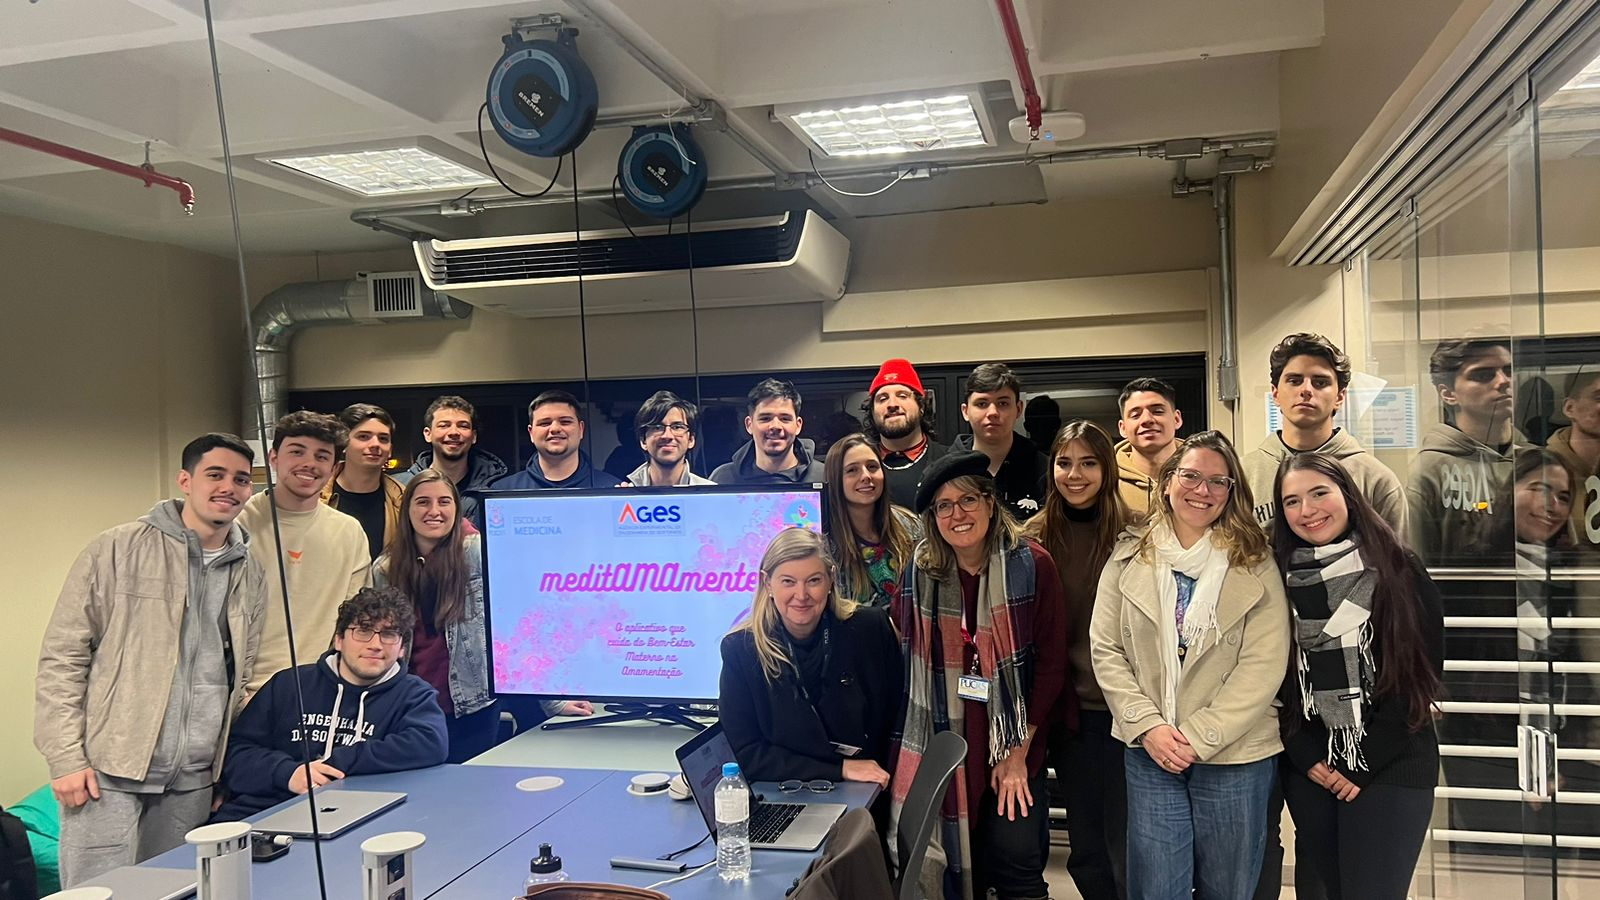
\includegraphics[width=1\linewidth]{conteudo/3 - ages II/conteudo/figures/foto-do-time.jpg}
    \label{fig:projeto-time-medita}
    \href{https://tools.ages.pucrs.br/meditamamente/wiki/-/wikis/home}{\textit{Fonte: https://tools.ages.pucrs.br/meditamamente/wiki/-/wikis/home}}
\end{figure}